% a tikz figure for HMM

\usetikzlibrary{shapes}

\tikzstyle{state}=[shape=circle,draw=blue!50,fill=blue!20]
\tikzstyle{observation}=[regular polygon,regular polygon sides=4,inner sep=1pt,draw=orange!50,fill=orange!20]
\tikzstyle{lightedge}=[<-,dotted]
\tikzstyle{mainstate}=[state,thick]
\tikzstyle{mainedge}=[<-,thick]

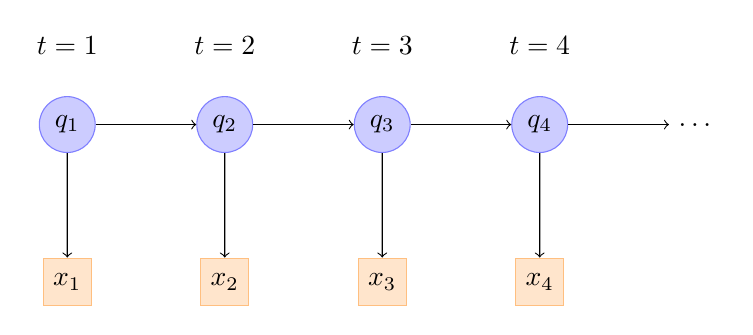
\begin{tikzpicture}[]
% time
  \node             at (0,3) {$t=1$};
  \node             at (2,3) {$t=2$};
  \node             at (4,3) {$t=3$};
  \node             at (6,3) {$t=4$};
% states
  \node[state] (q1) at (0,2) {$q_1$};
  \node[state] (q2) at (2,2) {$q_2$}
    edge [<-] (q1);
  \node[state] (q3) at (4,2) {$q_3$}
    edge [<-] (q2);
  \node[state] (q4) at (6,2) {$q_4$}
    edge [<-] (q3);
  \node             at (8,2) {\ldots}
    edge [<-] (q4);
% observations
  \node[observation] (x1) at (0,0) {$x_1$}
    edge [<-] (q1);
  \node[observation] (x2) at (2,0) {$x_2$}
    edge [<-] (q2);
  \node[observation] (x3) at (4,0) {$x_3$}
    edge [<-] (q3);
  \node[observation] (x3) at (6,0) {$x_4$}
    edge [<-] (q4);
\end{tikzpicture}

